\documentclass[border=0pt]{standalone}
\usepackage{fontspec}
\setmainfont{Carlito}
\usepackage{unicode-math}
\setmathfont{Latin Modern Math}
\usepackage{xcolor}
\usepackage{booktabs}
\usepackage{tikz}
\usepackage{graphicx}

\definecolor{canvabg}{RGB}{246,244,241}
\definecolor{textDark}{RGB}{40,40,40}
\definecolor{textMute}{RGB}{125,120,113}
\definecolor{accent}{RGB}{18,125,108}
\definecolor{trough}{RGB}{160,55,50}
\definecolor{bridge}{RGB}{30,90,140}

\pagecolor{canvabg}

\providecommand{\Cref}[1]{}
\providecommand{\cref}[1]{}
\providecommand{\ab}[1]{#1}

\renewcommand{\arraystretch}{1.2}

\begin{document}
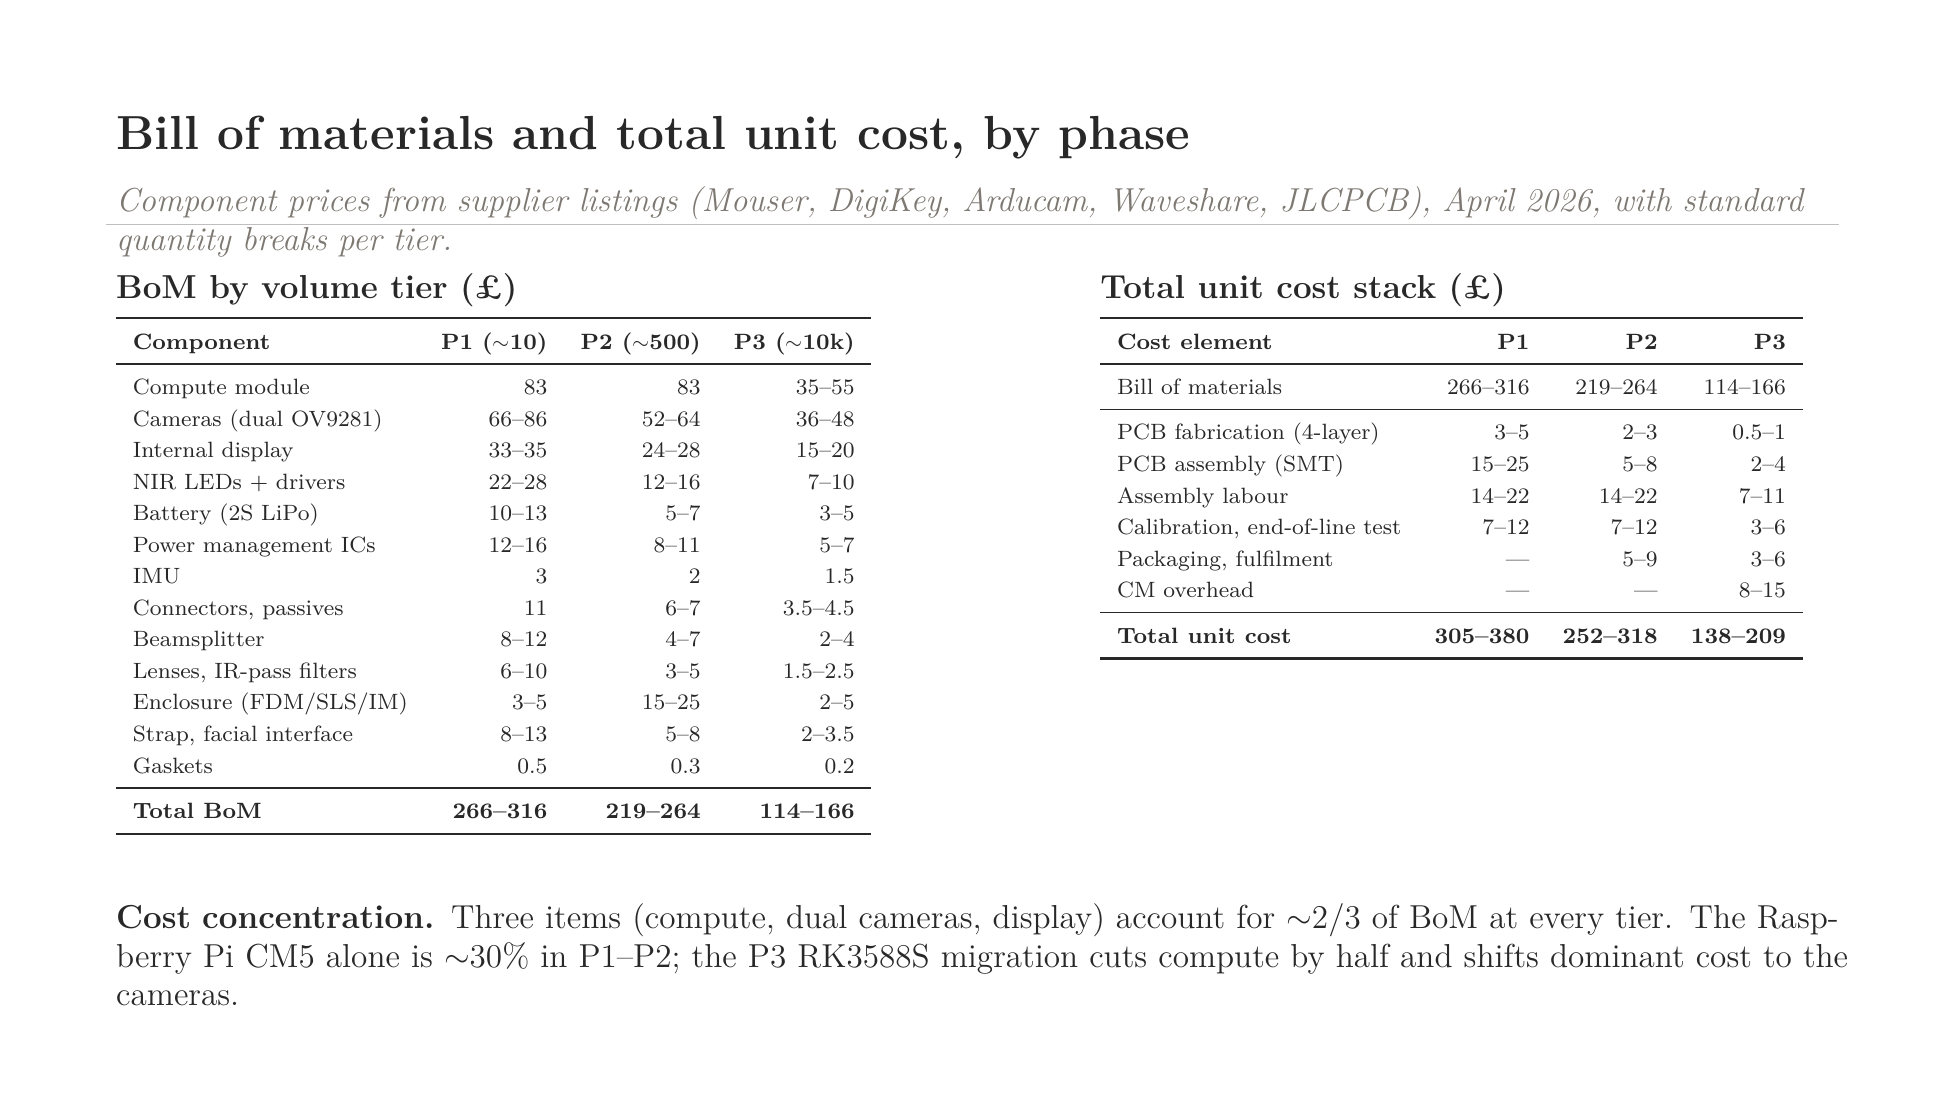
\begin{tikzpicture}[every node/.style={text=textDark}]
\useasboundingbox (0,0) rectangle (24, 13.5);

\node[anchor=north west, font=\bfseries\LARGE] at (1.0, 12.5)
    {Bill of materials and total unit cost, by phase};
\node[anchor=north west, font=\itshape\large, text=textMute, text width=22cm]
    at (1.0, 11.6)
    {Component prices from supplier listings (Mouser, DigiKey, Arducam, Waveshare,
     JLCPCB), April 2026, with standard quantity breaks per tier.};

\draw[gray!50, line width=0.5pt] (1.0, 11.0) -- (23.0, 11.0);

% BoM table on left
\node[anchor=north west, font=\bfseries\large] at (1.0, 10.5) {BoM by volume tier (\pounds)};
\node[anchor=north west, font=\footnotesize] at (1.0, 9.95) {%
\begin{tabular}{lrrr}
    \toprule
    \textbf{Component} & \textbf{P1 ($\sim$10)} & \textbf{P2 ($\sim$500)} & \textbf{P3 ($\sim$10k)} \\
    \midrule
    Compute module           & 83        & 83      & 35--55    \\
    Cameras (dual OV9281)    & 66--86    & 52--64  & 36--48    \\
    Internal display         & 33--35    & 24--28  & 15--20    \\
    NIR LEDs + drivers       & 22--28    & 12--16  & 7--10     \\
    Battery (2S LiPo)        & 10--13    & 5--7    & 3--5      \\
    Power management ICs     & 12--16    & 8--11   & 5--7      \\
    IMU                      & 3         & 2       & 1.5       \\
    Connectors, passives     & 11        & 6--7    & 3.5--4.5  \\
    Beamsplitter             & 8--12     & 4--7    & 2--4      \\
    Lenses, IR-pass filters  & 6--10     & 3--5    & 1.5--2.5  \\
    Enclosure (FDM/SLS/IM)   & 3--5      & 15--25  & 2--5      \\
    Strap, facial interface  & 8--13     & 5--8    & 2--3.5    \\
    Gaskets                  & 0.5       & 0.3     & 0.2       \\
    \midrule
    \textbf{Total BoM}     & \textbf{266--316} & \textbf{219--264} & \textbf{114--166} \\
    \bottomrule
\end{tabular}
};

% Total unit cost stack on right
\node[anchor=north west, font=\bfseries\large] at (13.5, 10.5) {Total unit cost stack (\pounds)};
\node[anchor=north west, font=\footnotesize] at (13.5, 9.95) {%
\begin{tabular}{lrrr}
    \toprule
    \textbf{Cost element} & \textbf{P1} & \textbf{P2} & \textbf{P3} \\
    \midrule
    Bill of materials              & 266--316 & 219--264 & 114--166 \\
    \midrule
    PCB fabrication (4-layer)      & 3--5     & 2--3     & 0.5--1   \\
    PCB assembly (SMT)             & 15--25   & 5--8     & 2--4     \\
    Assembly labour                & 14--22   & 14--22   & 7--11    \\
    Calibration, end-of-line test  & 7--12    & 7--12    & 3--6     \\
    Packaging, fulfilment          & ---      & 5--9     & 3--6     \\
    CM overhead                    & ---      & ---      & 8--15    \\
    \midrule
    \textbf{Total unit cost}     & \textbf{305--380} & \textbf{252--318} & \textbf{138--209} \\
    \bottomrule
\end{tabular}
};

% Reading note
\node[anchor=north west, text width=22cm, font=\large] at (1.0, 2.5)
    {\textbf{Cost concentration.} Three items (compute, dual cameras,
     display) account for $\sim$2/3 of BoM at every tier. The Raspberry Pi
     CM5 alone is $\sim$30\% in P1--P2; the P3 RK3588S migration cuts
     compute by half and shifts dominant cost to the cameras.};

\end{tikzpicture}
\end{document}
